%%%%%%%%%%%%%%%%%%%%%%%%%%%%%%%%%%%%%%%%%%%%%%%%%%%%%%%%%%%%%%%%%%%%%%%%%%%%%%%
%%  LensJudge -- the residual-image transformation (old vs new).
%%  Standalone report (sibling of main.tex). Figures from
%%  ../eval/make_residual_figures.py; the residual code is in common/render.py;
%%  the honesty tests are in tests/test_residual_honesty.py.
%%%%%%%%%%%%%%%%%%%%%%%%%%%%%%%%%%%%%%%%%%%%%%%%%%%%%%%%%%%%%%%%%%%%%%%%%%%%%%%
\documentclass[11pt,letterpaper]{article}
\usepackage{../../tech-report}
\usepackage{graphicx}

\newcommand{\lj}{\textsc{LensJudge}}
\newcommand{\plens}{\ensuremath{p_{\mathrm{lens}}}}
\newcommand{\chisig}{\ensuremath{\chi=(\mathrm{data}-\mathrm{model})/\sigma}}

\title{An Honest Residual Image for Strong-Lens Vetting:\\
       From a Gaussian High-Pass to a Signed, Noise-Normalized\\
       Elliptical-Model Residual in \lj{}}
\author{Greg Benson\thanks{\texttt{benson@cs.usfca.edu}; Department of Computer
        Science, University of San Francisco, CA 94117, USA} \and
        Xiaosheng Huang\thanks{Department of Physics \& Astronomy, University of
        San Francisco; and Physics Division, Lawrence Berkeley National Laboratory}}
\date{June 2026}
\addbibresource{references.bib}

\begin{document}
\maketitle
\subtitle{Why the old residual could both fabricate and hide arc flux, what replaced it, how it was validated, and what a controlled A/B shows it does (and does not) do to grading}

\begin{abstract}
The \lj{} vetting cascade shows a Claude grader a small set of rendered views of each candidate's DESI
\emph{grz} cutout; the ``residual'' view --- the smooth lens-galaxy light removed so that lensed arcs stand out
--- is the most error-prone to compute and one of the most influential, since it is returned to the model on
\emph{every} grading call. The original residual was a per-band Gaussian high-pass, re-floored to non-negative and
shown as an arcsinh RGB. We show that this transformation is \emph{not honest to the raw data} in four concrete
ways: it destroys the sign of the residual (hiding over-subtraction), it imprints a four-lobe ``butterfly''
quadrupole on elliptical galaxies that mimics arcs, it carries no noise normalization, and its kernel scale is
comparable to the seeing so it subtracts real arc flux and rings every compact source. We replace it with a
\emph{signed, noise-normalized, elliptical-model residual}: per band, a sigma-clipped median over elliptical
annuli (matched to the galaxy's ellipticity and position angle) is subtracted from the seeing-convolved data
without deconvolution, the residual is divided by a robust per-band noise $\sigma$, and the dimensionless
$\chi=(\mathrm{data}-\mathrm{model})/\sigma$ is displayed on a fixed $\pm5\sigma$ red--blue diverging scale as a
$g\,|\,r\,|\,z$ montage. Nothing is re-floored or clipped, so over-subtraction stays visible; the median rejects a
minority-fill arc so it survives in the residual; cross-band coherence becomes the discriminant between a real arc
and a per-pixel artifact. We document the design choices (median model as the default, with a photutils
elliptical-isophote engine as an opt-in --- it converges on under $15\%$ of these faint cutouts; and the
median over a more flexible harmonic fit that would \emph{absorb} real rings), and validate the new residual on
synthetic galaxies: outside the inner $\sim$2\arcsec\ the residual is consistent with $\mathcal{N}(0,1)$, an
injected arc is recovered at $0.63$ of its in-mask flux versus $0.08$ for the old high-pass, the smooth-galaxy
residual is $7\times$ smaller, and deliberate over-subtraction is plainly visible. The honest cost is a central
PSF-circularization residual confined to the inner $\sim$2\arcsec, shown faithfully as a blue core rather than
hidden. A controlled grading A/B on $525$ candidates then measured the downstream effect: the new residual is
\emph{discrimination-neutral} (lens-vs-random $\Delta\mathrm{AUC}=+0.021$, $95\%$ CI $[-0.04,+0.09]$); it exposed
and let us fix a real regression in the grader's residual \emph{convention} (an early ``blue $=$ artifact'' wording
made the grader reject real, blue arcs); and because the new image makes the grader score $\sim$$2\times$ hotter, it
must be deployed through an operating-point calibration, not its raw grade. The gain is integrity and defensibility,
not grading accuracy.
\end{abstract}

\section{The residual view, and why it must be honest}
\lj{} grades a strong-lens candidate from a handful of rendered views of its $101$-px \emph{grz} cutout
($0.262\arcsec$/px). The Claude SDK has no image-in-prompt channel, so these PNGs --- returned by the
\texttt{fetch\_cutout} tool --- are the \emph{only} way the model sees pixels. Three views are shown by default:
the full Lupton-RGB cutout, a $2.5\times$ center zoom, and the \emph{residual}, in which the smooth deflector
galaxy is removed so that a faint lensed arc or Einstein ring can stand out against the much brighter foreground.
The residual is therefore not decoration: it is evidence the automated grader reasons over on every call, and it
also appears as a figure panel in the published candidate galleries.

A residual image is honest to the raw data when it \emph{introduces no feature the data lacks and hides none that
exist}. Concretely this means: it preserves the sign of the residual (excess flux and over-subtraction are
equally informative), it carries a meaning in units of noise (so ``how significant'' is legible), it subtracts a
defensible model of the smooth galaxy rather than an arbitrary spatial filter, and it does not manufacture
arc-like structure where the sky has none. The original \lj{} residual violated all four of these. We diagnose
the failures (\S\ref{sec:old}), describe the replacement (\S\ref{sec:new}), compare them on real cutouts
(\S\ref{sec:compare}), justify the design (\S\ref{sec:design}), and validate it (\S\ref{sec:valid}).

\section{The old transformation and its four failures}
\label{sec:old}
The original residual (\texttt{render.residual\_legacy}, retained for reproducibility) was, per band $b\in\{g,r,z\}$,
a difference of the data and an isotropic Gaussian-smoothed copy, then re-floored to non-negative and rendered as
a reduced-stretch Lupton arcsinh RGB \citep{lupton2004}:
\[
  \mathrm{res}_b = \mathrm{data}_b - \mathcal{G}_{\sigma=3}\!\left[\mathrm{data}_b\right],\qquad
  \mathrm{res} \leftarrow \mathrm{res} - \min(\mathrm{res}).
\]
This has four distinct problems, each of which is either a hidden truth or a fabricated one.

\paragraph{(i) Sign destruction.} The step $\mathrm{res}\leftarrow\mathrm{res}-\min(\mathrm{res})$ maps the most
negative pixel to zero, so every pixel where the model exceeded the data --- i.e.\ every \emph{over-subtraction}
--- becomes a positive value indistinguishable from genuine excess. A too-aggressive model can then delete real
arc flux with no visible trace. Over-subtraction is not a corner case: it is exactly what happens at the bright
galaxy core, and the re-floor renders it invisible (Fig.~\ref{fig:signnoise}, left).

\paragraph{(ii) The ``butterfly'' quadrupole.} A deflector is a relaxed elliptical galaxy, but an isotropic
Gaussian smoothing is circular. Subtracting a circular model from an elliptical galaxy leaves a four-lobe
quadrupole: a positive excess along the major axis (which \emph{mimics a tangential arc}) and a negative trough
along the minor axis (which \emph{erases} real flux there). Figure~\ref{fig:butterfly} shows this directly on a
synthetic elliptical galaxy. This is the most insidious failure: the artifact looks like the signal.

\paragraph{(iii) No noise normalization.} The output is in arbitrary counts passed through an arcsinh stretch.
Two consequences follow. First, the viewer (human or model) cannot tell a $5\sigma$ feature from a $1\sigma$ one.
Second, an arcsinh RGB cannot represent negative numbers at all, which is \emph{why} step (i) is needed in the
first place --- the display format forces the dishonesty.

\paragraph{(iv) Scale comparable to the seeing.} The kernel $\sigma=3$\,px is $\approx0.79\arcsec$, comparable to
the $\sim$$1.2\arcsec$ DECam PSF. A high-pass at the seeing scale subtracts real arc flux (the arc is itself only
marginally resolved) and imprints a Mexican-hat ring around every compact source. Features in such a residual are
partly manufactured by the filter, not present in the sky.

\begin{figure}[t]\centering
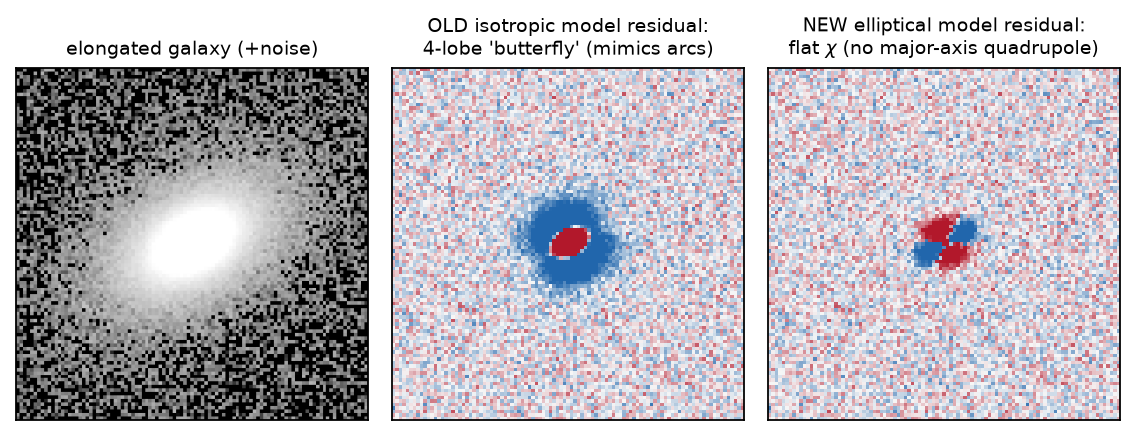
\includegraphics[width=0.92\linewidth]{figures/resid_butterfly.png}
\caption{The butterfly artifact (failure ii), on a synthetic elliptical galaxy with noise. \emph{Left}: the
galaxy. \emph{Middle}: the old isotropic-model residual $\mathrm{data}-\mathcal{G}_{\sigma=3}[\mathrm{data}]$,
shown on the new signed scale at the same noise level --- a strong central quadrupole (red along the major axis,
blue along the minor), the lobes of which masquerade as arcs. \emph{Right}: the new elliptical-model residual on
the same data --- flat noise, no major-axis quadrupole. Red is positive (excess), blue negative
(over-subtraction).}
\label{fig:butterfly}
\end{figure}

\section{The new transformation: a signed, noise-normalized elliptical residual}
\label{sec:new}
The replacement (\texttt{render.residual}) is built in three stages: model, noise, display
(Fig.~\ref{fig:anatomy}).

\paragraph{Model.} For each band we subtract a smooth model of the galaxy formed as a \emph{sigma-clipped median
over elliptical annuli}. The galaxy's center, ellipticity, and position angle are estimated once from the
sigma-clipped second moments of the $r{+}z$ luminance; pixels are binned into one-pixel-wide elliptical annuli of
that geometry, and each annulus is assigned its sigma-clipped median. Three properties make this honest. It
carries the galaxy's true ellipticity and orientation, so it leaves no butterfly. It is fit to, and subtracted in,
the \emph{seeing-convolved} data --- there is no deconvolution, so the model is automatically PSF-matched, which
matters because the cutouts carry no stored PSF. And because it is a \emph{median}, a tangential arc that fills a
minority of an annulus barely moves the model and therefore survives in the residual, whereas a least-squares or
mean model would be dragged toward the arc and partly cancel it. The elliptical-annulus median is the
azimuthally-resolved generalization of the circular profiles long used for galaxy photometry
\citep{jedrzejewski1987}, and is exactly the smooth-model recipe (median integration, $3\sigma$ clipping) the
Siena Galaxy Atlas applies to Legacy Survey \emph{grz} imaging at scale \citep{moustakas2023sga}.

\paragraph{Noise.} We divide by a robust per-band noise $\sigma$, the median-absolute-deviation standard
deviation (\texttt{mad\_std}) of the $3\sigma$-clipped residual, cross-checked against the frame border; the
sigma-clip rejects the arc and the galaxy core, so $\sigma$ measures sky plus correlated noise. The displayed
quantity is the dimensionless \chisig{}.

\paragraph{Display.} $\chi$ is rendered on a fixed $\pm5\sigma$ red--blue diverging scale (red positive, blue
negative, white at zero), arcsinh-compressed within the range, as a horizontal $g\,|\,r\,|\,z$ montage. Nothing is
re-floored or clipped, so over-subtraction remains visible as blue. The fixed limits make every object directly
comparable. The bands are shown separately because \emph{cross-band coherence is the discriminant}: a real lensed
arc is a connected feature present in $g$ and $r$ (the source is blue, so it is strong in $g/r$ and weak in $z$),
whereas per-pixel noise and model-mismatch rings are not band-coherent. Crucially, the discriminant is \emph{shape
and cross-band coherence, not the residual's sign}: because the source is blue and a single-elliptical subtraction
can leave a real arc either red or blue, a viewer (or grader) must never equate ``blue'' with ``artifact'' --- a
lesson \S\ref{sec:grading} learned the hard way. We never pass the residual through the Lupton transform, which
cannot show negative values \citep{lupton2004}.

\begin{figure}[t]\centering
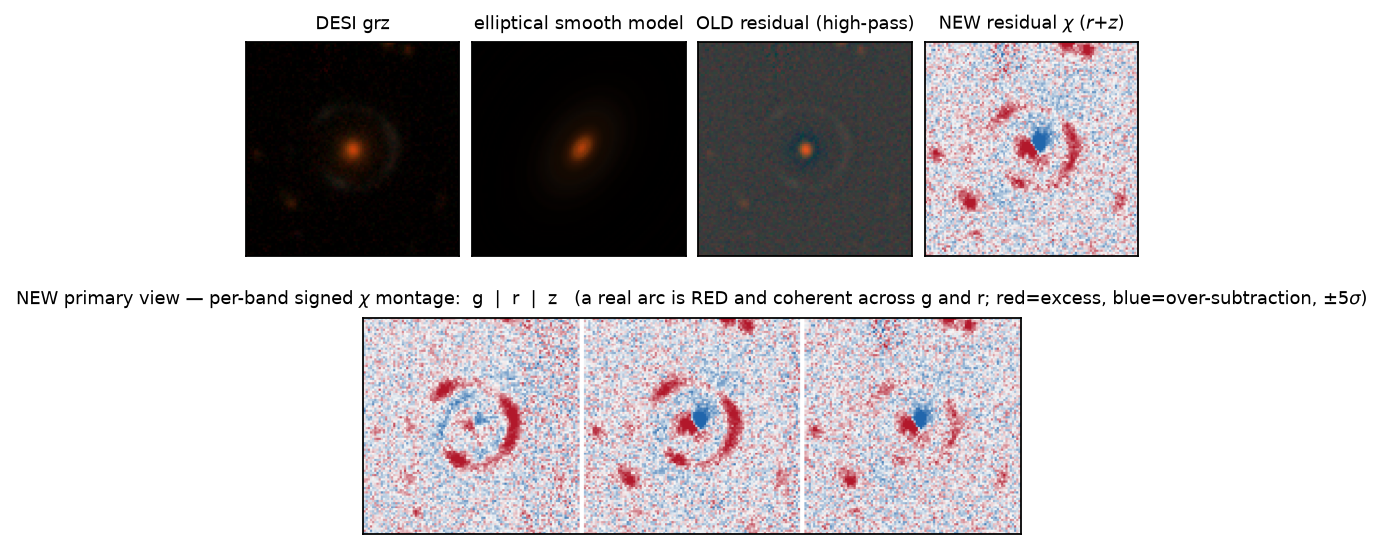
\includegraphics[width=0.98\linewidth]{figures/resid_anatomy.png}
\caption{Anatomy of the new residual on the Cosmic Horseshoe (CSWA~1). \emph{Top, left to right}: the DESI
\emph{grz} cutout; the elliptical smooth-light model that is subtracted; the old high-pass residual (washed out by
the re-floor and arcsinh); and the new single-panel $\chi$ of the $r{+}z$ luminance. \emph{Bottom}: the new
primary view shown to the grader --- the per-band signed-$\chi$ montage, in which the Einstein ring is red and
coherent across $g$ and $r$, with a blue (honestly displayed) over-subtracted core.}
\label{fig:anatomy}
\end{figure}

\section{Side-by-side comparison on real candidates}
\label{sec:compare}
Figure~\ref{fig:examples} is the central comparison: the old and new residuals on the \emph{same} DECam cutouts of
four DR11 systems. The two rows of known lenses show the new residual revealing a red, cross-band-coherent arc
(a near-complete ring for CSWA~1; a tangential arc for the Huang+2020 system), with the over-subtracted core
honestly visible in blue. The two rows of \texttt{lrg+companion} \emph{mimics} --- candidates the finder ranked
highly but which are not lenses --- show the new residual surfacing the companion as a compact blob, \emph{not}
the tangential arc a genuine lens produces; the morphology, read across bands, is what separates them. In every
row the old residual is a muddy blob with a high-pass ring around the core, conveying essentially nothing the
grader can use. The same transformation that makes a real arc legible also refuses to manufacture one where the
sky has only a companion galaxy.

\begin{figure}[t]\centering
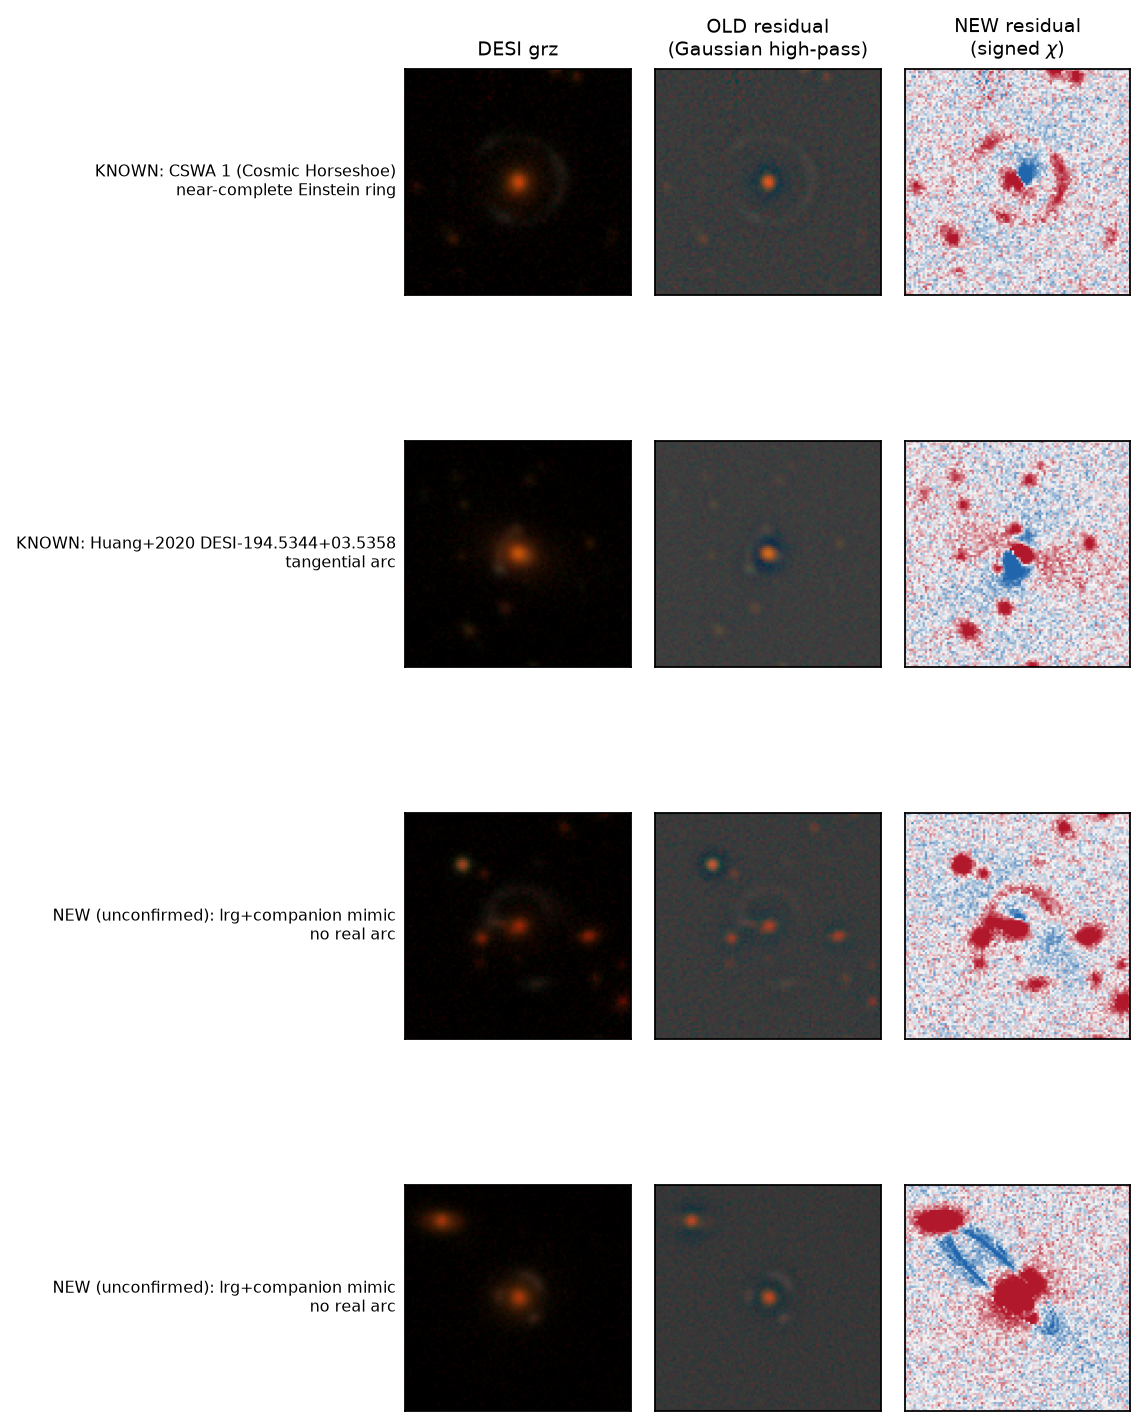
\includegraphics[width=0.86\linewidth]{figures/resid_examples.png}
\caption{Old vs new residual on identical DESI cutouts (rows: two known lenses, two \texttt{lrg+companion}
mimics). \emph{Left}: DESI \emph{grz}. \emph{Middle}: the old Gaussian high-pass residual --- uniformly muddy,
with a ring artifact. \emph{Right}: the new signed-$\chi$ residual ($r{+}z$ luminance) --- a red arc for the
lenses, only noise/blobs for the mimics. The new residual both \emph{reveals} real arcs and \emph{declines to
fabricate} them.}
\label{fig:examples}
\end{figure}

\section{Design choices, and what we deliberately did not do}
\label{sec:design}
\paragraph{Median model by default; isophote fitting as an opt-in.} A floating elliptical-\emph{isophote} fit
\citep{jedrzejewski1987}, which lets ellipticity and position angle vary with radius, is in principle more
faithful and is available as an opt-in engine (\texttt{photutils.isophote} \citep{bradley_photutils}). In practice
it converges on fewer than $15\%$ of these faint $101$-px \emph{grz} cutouts and is $10$--$50\times$ slower, so on
this data it would mostly fall back anyway; the elliptical-annulus median is the fast, always-converging default,
with the isophote engine reserved for higher signal-to-noise imaging (HSC/Euclid). A multi-Gaussian expansion
\citep{cappellari2002mge} is a third, strictly-positive option in the same spirit.

\paragraph{Median over a more flexible fit --- ``under-fit on purpose''.} A natural ``improvement'' is to fit
low-order azimuthal harmonics per annulus, which removes the central PSF-circularization residual. It also
\emph{absorbs real arcs}: Figure~\ref{fig:tradeoff} shows that on the Cosmic Horseshoe an aggressive harmonic fit
eats the Einstein ring, while the median preserves it. Because every added degree of freedom can absorb a lensed
feature \citep{peng2010galfit}, and because near-complete rings are exactly the most spectacular lenses, we
deliberately under-fit: the median leaves an honest central residual rather than risk deleting the signal. This is
the same lesson that motivates b-spline lens-galaxy subtraction in the SLACS program \citep{bolton2006slacs} and
the ``no lens left behind'' principle of \emph{modelling} the source rather than masking it in forward fitting
\citep{etherington2022}. The rigorous endpoint --- a full forward model of lens, source, and PSF with a
$\chi$ residual \citep{birrer2021lenstronomy} --- is the right tool for confirmation but is overkill for an
unattended quick-look view over hundreds of cutouts.

\begin{figure}[t]\centering
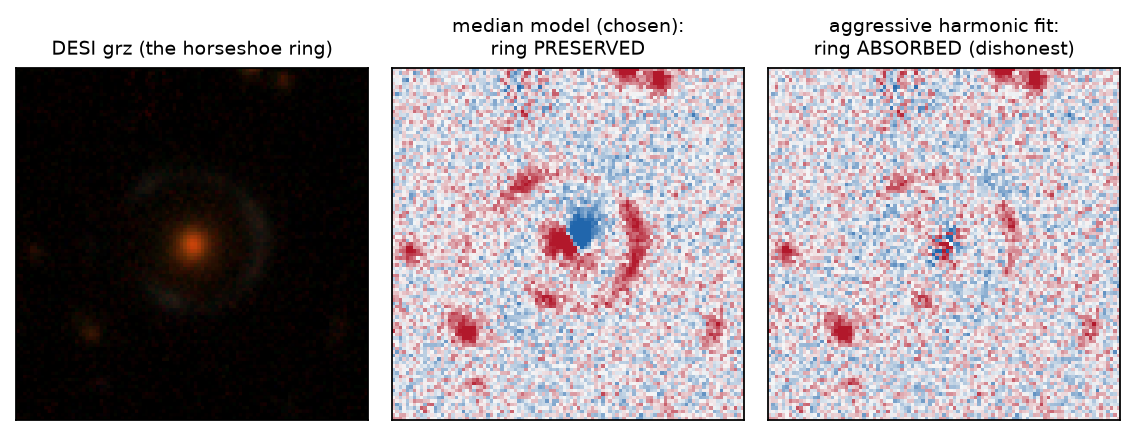
\includegraphics[width=0.86\linewidth]{figures/resid_tradeoff.png}
\caption{Why we under-fit. \emph{Left}: the horseshoe in DESI \emph{grz}. \emph{Middle}: the chosen median model
--- the ring is preserved. \emph{Right}: an aggressive per-annulus harmonic fit --- the same ring is absorbed into
the model and vanishes from the residual. A vanishing residual is a red flag, not a success.}
\label{fig:tradeoff}
\end{figure}

\section{Validation}
\label{sec:valid}
Four synthetic tests (\texttt{tests/test\_residual\_honesty.py}), each building a PSF-convolved S\'ersic galaxy
($\sim$$1.2\arcsec$ FWHM) with noise matched to a real cutout, check the four properties the old residual
violated; all pass. \textbf{(1) Noise consistency:} outside the inner $\sim$2\arcsec\ the residual $\chi$ is
consistent with $\mathcal{N}(0,1)$ (mean $0.00$, standard deviation $0.99$, $0.32\%$ of pixels beyond $3\sigma$
versus the Gaussian expectation $0.27\%$), with no coherent structure --- no butterfly. \textbf{(2) Arc
non-absorption:} an injected tangential arc is recovered at $0.63$ of its in-mask flux, against $0.08$ for the old
Gaussian high-pass. \textbf{(3) Sign preservation:} a deliberate $5\%$ over-subtraction produces a clearly visible
negative (blue) bowl that the old re-floor would have hidden (Fig.~\ref{fig:signnoise}). \textbf{(4) Smooth-galaxy
modelling:} on an elongated galaxy the elliptical model's residual outside the core is $7\times$ smaller than the
old high-pass's, and is core-confined (it falls steeply with radius). The new residual costs about $40$\,ms per
object and never fails to produce an image.

\begin{figure}[t]\centering
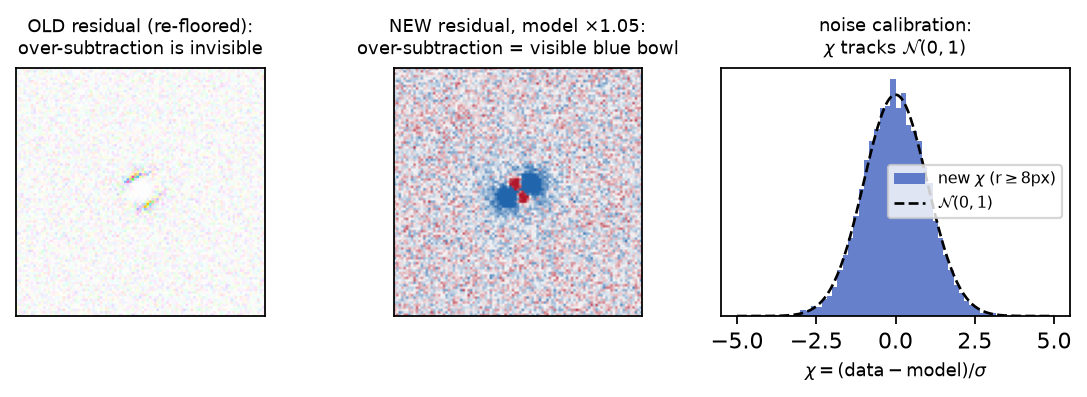
\includegraphics[width=0.98\linewidth]{figures/resid_sign_noise.png}
\caption{Sign and noise (validation tests 1 and 3). \emph{Left}: the old residual re-floors, so an
over-subtraction is invisible. \emph{Middle}: the new residual of the same galaxy with the model scaled up $5\%$
--- the over-subtraction is a plainly visible blue bowl. \emph{Right}: the new residual $\chi$ outside the inner
core tracks $\mathcal{N}(0,1)$, so a pixel value reads directly as a significance.}
\label{fig:signnoise}
\end{figure}

\section{Does it change grading? A controlled A/B}
\label{sec:grading}
The honesty tests above measure the residual against the \emph{pixels}; they do not measure its effect on the
downstream judgement. To do that we ran a controlled A/B that grades the \emph{same} candidates twice, swapping only
the residual view (old vs new) through a single environment lever (\texttt{LENSJUDGE\_RESIDUAL\_VERSION}, read by
\texttt{render.render\_views} and \texttt{residual\_view\_desc}); everything else --- the full/zoom views, the
rubric, the model --- is held fixed. We graded $525$ candidates with the deployed direct grader: $240$
expert-graded A/B/C lenses, $130$ Grade-D human-rejects (the hardest negatives), $130$ random galaxies, and $25$
spectroscopically-confirmed ``gold'' systems; two replicates per arm. The primary endpoint is the threshold-free
ROC-AUC with a paired bootstrap CI; because the residual's prompt wording shifts the grader's operating point (see
below), we also compare at a \emph{matched} false-positive rate (Table~\ref{tab:ab}).

\paragraph{It is discrimination-neutral.} On the core detection task (lens vs random galaxy) the new residual does
not measurably improve the grader: $\Delta\mathrm{AUC}=+0.021$ with a $95\%$ CI of $[-0.043,+0.085]$ that straddles
zero (Fig.~\ref{fig:abresults}a), and at a matched $\mathrm{FPR}=0.2$ the grade-A recall is \emph{identical}
($0.256$ in both arms). The large uncalibrated recall ``gains'' are a uniform threshold shift, not better
separation (below), and they vanish once the FPR is matched. On the hardest negatives (lens vs Grade-D) the new
residual is significantly \emph{less bad} ($\Delta\mathrm{AUC}=+0.076$, CI $[+0.017,+0.140]$), but both arms sit
\emph{below} $0.5$: the grader still ranks human-rejected look-alikes above real lenses, so this is ``less wrong,''
not usable discrimination.

\paragraph{A regression we caught, and the lesson.} The A/B exposed a real harm in the residual's \emph{prompt
convention}, not its pixels. Our first deployed wording told the grader ``red $=$ arc, blue $=$ over-subtraction
artifact.'' But a lensed source is blue, and after a single-elliptical subtraction a genuine arc often renders blue,
so the grader --- conflating the residual's \emph{sign} with the source's \emph{colour} --- re-read real grade-A
arcs as artifacts and rejected them (grade-A recall fell $0.259\!\to\!0.185$). Rewriting the description to be
morphology-first (judge a \emph{tangential, cross-band-coherent} feature offset from the over-subtracted inner
$\sim$2\arcsec\ core; never treat blue as an artifact) restored grade-A non-inferiority. The residual's prompt is
load-bearing: it must key on shape and cross-band coherence, never on sign.

\paragraph{Hotter scores demand calibration.} The new residual inflates \plens{} roughly $2\times$ across the board;
used raw it floods false positives (random-galaxy FPR $0.12\!\to\!0.30$, Grade-D $0.27\!\to\!0.49$;
Fig.~\ref{fig:abresults}b) while the ROC-AUC barely moves --- a pure operating-point shift. We therefore ship the
new residual with an FPR-matched operating point (\texttt{eval/calibrate.py}: a \plens{} threshold fit to a target
FPR on a labelled negative set, persisted as \texttt{residual\_op\_point\_*.json}). Calibrated, the flood is removed
and both arms sit at one operating point, where their grade-A recall coincides (Fig.~\ref{fig:abresults}c). The
decision must use the calibrated threshold, never the raw grade.

\begin{table}[t]\centering
\caption{The residual A/B (legacy old residual vs the new signed-$\chi$ residual; $525$ candidates, two replicates
per arm). AUC is the threshold-free primary endpoint with a paired bootstrap $95\%$ CI; recall and FPR are at, or
calibrated to, a matched operating point. The change is discrimination-neutral, preserves grade-A at a matched FPR,
and needs calibration to control the false-positive flood.}
\label{tab:ab}\small
\begin{tabular}{lcc}
\toprule
quantity & legacy & new\\
\midrule
AUC, lens vs random                      & $0.650\,[0.59,0.70]$ & $0.671\,[0.61,0.72]$\\
\quad$\Delta$AUC (new$-$legacy)          & \multicolumn{2}{c}{$+0.021\,[-0.043,+0.085]$ (n.s.)}\\
AUC, lens vs Grade-D                     & $0.387$ & $0.463$ (both $<0.5$)\\
grade-A recall @ matched FPR$=0.2$       & $0.256$ & $0.256$\\
random-galaxy FPR (raw $\to$ calibrated) & $0.12\to0.12$ & $0.30\to0.12$\\
Grade-D FPR (raw $\to$ calibrated)       & $0.27\to0.28$ & $0.49\to0.35$\\
\bottomrule
\end{tabular}
\end{table}

\begin{figure}[t]\centering
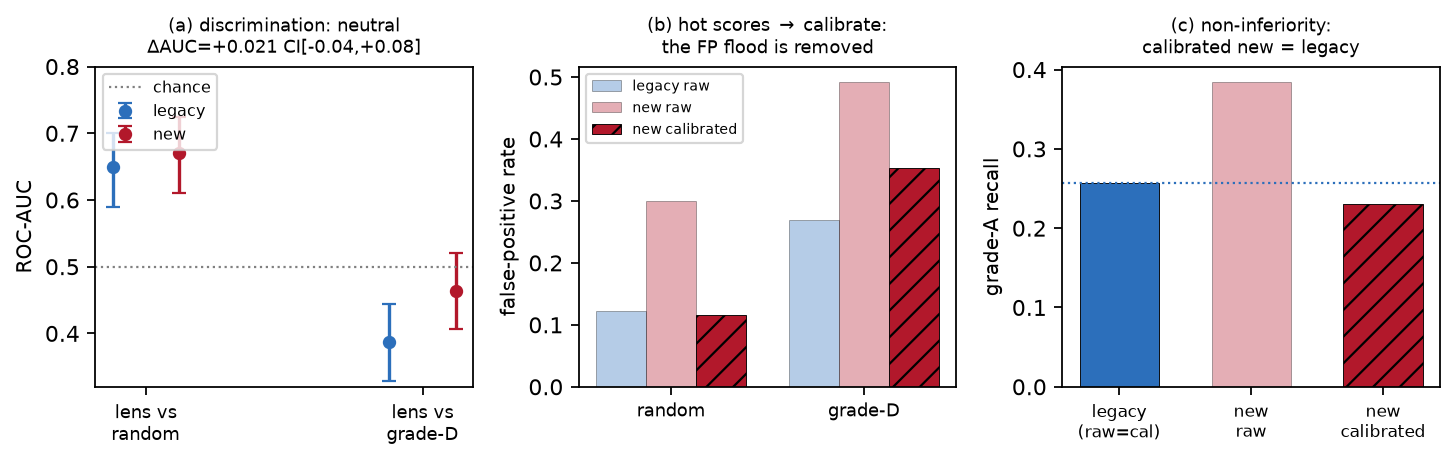
\includegraphics[width=0.98\linewidth]{figures/resid_ab_results.png}
\caption{The grading A/B. \emph{(a)} ROC-AUC with bootstrap $95\%$ CIs: the arms overlap on lens-vs-random (the
$\Delta$AUC CI includes $0$), and both are below chance on lens-vs-Grade-D. \emph{(b)} Negative false-positive
rate: the new residual's raw scores flood FPs; the FPR-matched calibration removes it. \emph{(c)} grade-A recall:
the new arm runs hot (raw), but calibrated it equals legacy --- non-inferiority at the matched operating point.}
\label{fig:abresults}
\end{figure}

\paragraph{What it is worth.} The honest bottom line: the new residual is a \emph{scientific-integrity} improvement
that is \emph{grading-discrimination-neutral}. Its benefits are a defensible, sign-preserving, noise-normalized
image; rationales that key on real morphology; and decisive upgrades of clean tangential arcs --- not a broad
accuracy gain, and at $\sim$$37\%$ more cost per call. Caveats: only two replicates per arm; grade-A ($n{=}39$) and
gold ($n{=}21$) are underpowered, and gold's matched-FPR recall trends down in a way the headline numbers hide; and
the artifact-rejection failure was \emph{reshaped, not removed} --- faint, blobby, or close-pair real lenses are
still sometimes dismissed as over-subtraction. These set the agenda for a larger, pre-registered follow-up.

\section{Limitations}
The honest residual is honest about its own limits. The cutouts carry \emph{no PSF and no inverse-variance map},
so the model is only as PSF-matched as the blurred data (a faint central image inside the Einstein radius can
still be partly absorbed), and the noise $\sigma$ is \emph{estimated}; because DESI coadds have spatially
correlated (resampled) noise, $\chi$ slightly under-estimates the uncertainty of a multi-pixel arc and should be
read as a display/triage significance, not a calibrated detection statistic. The single-ellipticity model leaves a
central PSF-circularization residual confined to the inner $\sim$2\arcsec, shown faithfully as a blue core that the
grader is told to \emph{ignore} rather than to read as an artifact verdict (the A/B of \S\ref{sec:grading} showed an
earlier ``blue $=$ artifact'' instruction backfired); a galaxy that is genuinely irregular or strongly
isophote-twisted will leave honest but structured residuals that a validity flag (e.g.\ \texttt{statmorph}
\citep{rodriguezgomez2019statmorph}) can gate. Finally, a near-complete
Einstein ring that fills most of an annulus is partly absorbed by \emph{any} azimuthal-median model and is the
case to escalate to a masked or forward-model fit. The imaging used here is the DESI Legacy Surveys DECam coadds
\citep{legacysurvey}; the same transformation is applied to the higher-resolution HSC and Euclid tier-2 residuals,
where the isophote engine becomes viable. Finally, the grader's raw \plens{} on the new residual is uncalibrated and
runs hot (\S\ref{sec:grading}), so any deployed decision must pass through the FPR-matched operating point, not the
raw grade.

\bibliographystyle{plainnat}
\bibliography{references}

\end{document}
